\documentclass[tikz,border=2pt]{standalone}
% Preámbulo común de los diagramas TikZ (misma paleta y letra que las notas)
\usepackage[T1]{fontenc}\usepackage[utf8]{inputenc}
\usepackage{libertinus}\usepackage{libertinust1math}
\usepackage[defaultsans,scale=0.92]{lato}
\usepackage{amsmath,amssymb,bm}
\usepackage{tikz}\usetikzlibrary{calc,positioning,arrows.meta,shapes.geometric,decorations.pathreplacing,decorations.pathmorphing,fit,backgrounds}
\definecolor{snlazul}{HTML}{1E5AA8}\definecolor{snlnoche}{HTML}{14213D}\definecolor{snlvioleta}{HTML}{6C4AB6}
\definecolor{snlcoral}{HTML}{D1495B}\definecolor{snlambar}{HTML}{E09F3E}\definecolor{snlverde}{HTML}{2A9D8F}
\definecolor{snlteal}{HTML}{0F7173}\definecolor{snlgris}{HTML}{5C677D}\definecolor{snlfondo}{HTML}{F4F6FA}
\tikzset{>={Stealth[length=2.2mm]},
  bloque/.style={draw=#1,fill=#1!8,thick,rounded corners=2pt,minimum height=11mm,minimum width=20mm,align=center,font=\small},
  bloque/.default=snlazul,
  suma/.style={draw=snlnoche,thick,circle,inner sep=0pt,minimum size=5mm},
  flecha/.style={->,thick,draw=snlnoche},
  etq/.style={font=\small,text=snlnoche},
  nota/.style={font=\footnotesize\sffamily,text=snlgris,align=center}}

\begin{document}
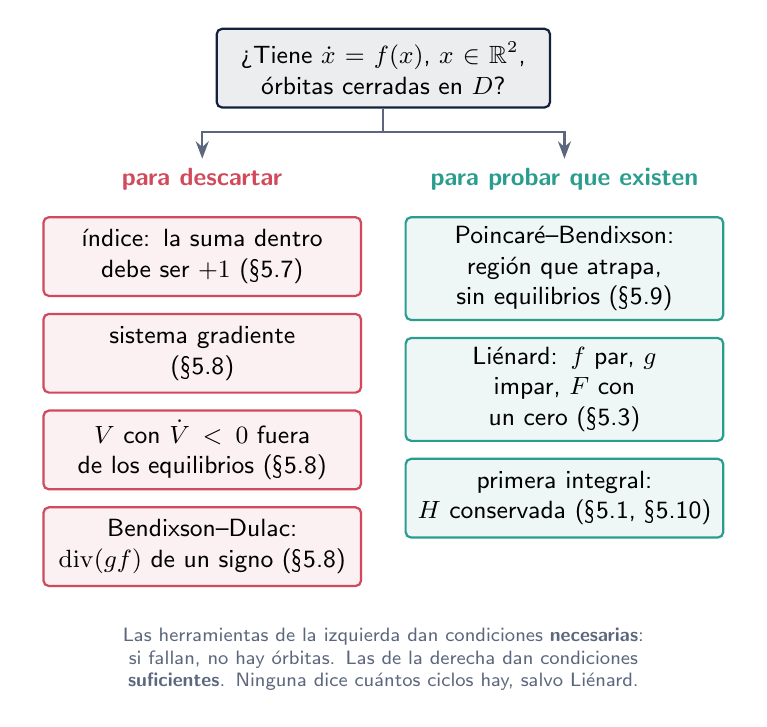
\begin{tikzpicture}[font=\sffamily\small,
  caja/.style={draw=#1,fill=#1!8,thick,rounded corners=2pt,align=center,minimum height=10mm,text width=38mm},
  tit/.style={font=\sffamily\bfseries\small,text=#1},
  fl/.style={-{Stealth[length=2.2mm]},thick,draw=snlgris}]
  \node[caja=snlnoche,text width=40mm] (q) {¿Tiene $\dot x=f(x)$, $x\in\mathbb{R}^2$,\\ órbitas cerradas en $D$?};
  % columna izquierda: descartar
  \node[tit=snlcoral] (tno) at ($(q.south)+(-23mm,-9mm)$) {para \emph{descartar}};
  \node[caja=snlcoral,below=2mm of tno] (ind) {índice: la suma dentro\\ debe ser $+1$ (\S5.7)};
  \node[caja=snlcoral,below=2mm of ind] (gra) {sistema gradiente\\ (\S5.8)};
  \node[caja=snlcoral,below=2mm of gra] (lya) {$V$ con $\dot V<0$ fuera\\ de los equilibrios (\S5.8)};
  \node[caja=snlcoral,below=2mm of lya] (ben) {Bendixson--Dulac:\\ $\operatorname{div}(gf)$ de un signo (\S5.8)};
  % columna derecha: probar existencia
  \node[tit=snlverde] (tsi) at ($(q.south)+(23mm,-9mm)$) {para \emph{probar} que existen};
  \node[caja=snlverde,below=2mm of tsi] (pb) {Poincaré--Bendixson:\\ región que atrapa,\\ sin equilibrios (\S5.9)};
  \node[caja=snlverde,below=2mm of pb] (lie) {Liénard: $f$ par, $g$\\ impar, $F$ con un cero (\S5.3)};
  \node[caja=snlverde,below=2mm of lie] (int) {primera integral:\\ $H$ conservada (\S5.1, \S5.10)};
  \draw[fl] (q.south) -- ++(0,-3mm) -| (tno.north);
  \draw[fl] (q.south) -- ++(0,-3mm) -| (tsi.north);
  \node[font=\sffamily\scriptsize,text=snlgris,align=center,below=4mm of ben,xshift=23mm,text width=88mm]
     {Las herramientas de la izquierda dan condiciones \textbf{necesarias}: si fallan, no hay órbitas.
      Las de la derecha dan condiciones \textbf{suficientes}. Ninguna dice cuántos ciclos hay, salvo Liénard.};
\end{tikzpicture}
\end{document}
